% ============================================================================
%  ECE 431 -- Sheet 5 Solutions
%  Style: sheet-answering-style.md
% ============================================================================

\begin{question}[Question 1]
Find an expression of electron and hole concentrations per unit energy $n(E)$ and $p(E)$ in bulk semiconductors. Sketch these concentrations as a function of energy. Derive an expression of the energies at which they attain their peak values in the case of non-degenerate semiconductors. Find the photon wavelength corresponding to radiative transition between these peaks in GaAs ($E_g = 1.42$ eV) at room temperature. Is this transition possible? Explain. Find the ratio of carrier concentration at $2K_BT$ from the band edge to the peak concentration.
\end{question}

\textbf{\large Solution --- Question 1}

\textbf{Carrier concentrations per unit energy.}

The density of states for electrons in the conduction band and holes in the valence band are given by:

\begin{equation*}
  S_e(E) = \frac{\sqrt{2} m_e^{* 3/2}}{\pi^2 \hbar^3} \sqrt{E - E_c} \quad \text{and} \quad S_h(E) = \frac{\sqrt{2} m_h^{* 3/2}}{\pi^2 \hbar^3} \sqrt{E_v - E}
\end{equation*}

For a non-degenerate semiconductor, the Fermi-Dirac distributions are approximated by the Boltzmann distribution:

\begin{equation*}
  f(E) \simeq \exp\left(-\frac{E-E_f}{k_B T}\right) \quad \text{and} \quad 1-f(E) \simeq \exp\left(\frac{E-E_f}{k_B T}\right)
\end{equation*}

The carrier concentrations per unit energy are the product of the density of states and the occupation probability:

\begin{equation*}
  \boxed{n(E) = S_e(E) f(E) = \frac{\sqrt{2} m_e^{* 3/2}}{\pi^2 \hbar^3} \sqrt{E - E_c} \exp\left(-\frac{E-E_f}{k_B T}\right)}
\end{equation*}

\begin{equation*}
  \boxed{p(E) = S_h(E) [1-f(E)] = \frac{\sqrt{2} m_h^{* 3/2}}{\pi^2 \hbar^3} \sqrt{E_v - E} \exp\left(\frac{E-E_f}{k_B T}\right)}
\end{equation*}

\textbf{Peak concentration energies.}

To find the energy $E_{max}$ at which $n(E)$ attains its peak, we set the derivative to zero:

\begin{equation*}
  \frac{\partial n}{\partial E} = \frac{\sqrt{2} m_e^{* 3/2}}{\pi^2 \hbar^3} \left[ \frac{\exp\left(-\frac{E-E_f}{k_B T}\right)}{2\sqrt{E-E_c}} - \frac{\exp\left(-\frac{E-E_f}{k_B T}\right)}{k_B T} \sqrt{E-E_c} \right] = 0
\end{equation*}

\begin{equation*}
  \frac{1}{2\sqrt{E-E_c}} = \frac{\sqrt{E-E_c}}{k_B T} \quad\Longrightarrow\quad \boxed{E_{max}^{(n)} = E_c + \frac{k_B T}{2}}
\end{equation*}

Substituting this back gives the peak electron concentration per unit energy:

\begin{equation*}
  n_{max} = n\left(E_c + \frac{k_B T}{2}\right) = \frac{\sqrt{k_B T} m_e^{* 3/2}}{\pi^2 \hbar^3} \exp\left(-\frac{E_c - E_f}{k_B T} - \frac{1}{2}\right)
\end{equation*}

Similarly, for holes:

\begin{equation*}
  \frac{\partial p}{\partial E} = \frac{\sqrt{2} m_h^{* 3/2}}{\pi^2 \hbar^3} \left[ \frac{-\exp\left(\frac{E-E_f}{k_B T}\right)}{2\sqrt{E_v-E}} + \frac{\exp\left(\frac{E-E_f}{k_B T}\right)}{k_B T} \sqrt{E_v-E} \right] = 0
\end{equation*}

\begin{equation*}
  \frac{1}{2\sqrt{E_v-E}} = \frac{\sqrt{E_v-E}}{k_B T} \quad\Longrightarrow\quad \boxed{E_{max}^{(p)} = E_v - \frac{k_B T}{2}}
\end{equation*}

And the peak hole concentration per unit energy:

\begin{equation*}
  p_{max} = p\left(E_v - \frac{k_B T}{2}\right) = \frac{\sqrt{k_B T} m_h^{* 3/2}}{\pi^2 \hbar^3} \exp\left(-\frac{E_f - E_v}{k_B T} - \frac{1}{2}\right)
\end{equation*}

\textbf{Peak transition wavelength and viability.}

The photon energy corresponding to the transition between these two peaks is:

\begin{equation*}
  h\nu = E_{max}^{(n)} - E_{max}^{(p)} = \left(E_c + \frac{k_B T}{2}\right) - \left(E_v - \frac{k_B T}{2}\right) = E_g + k_B T
\end{equation*}

For GaAs at room temperature ($E_g = 1.42$\,eV, $k_B T \approx 0.026$\,eV):

\begin{equation*}
  h\nu = 1.42 + 0.026 = 1.446\,\text{eV} \quad\Longrightarrow\quad \nu = \frac{1.446 \times 1.6\times10^{-19}}{6.626\times10^{-34}} \approx 3.49 \times 10^{14}\,\text{Hz}
\end{equation*}

\begin{equation*}
  \boxed{\lambda_{ph} = \frac{c}{\nu} \approx 0.86\,\mu\text{m}.}
\end{equation*}

Although we can calculate this wavelength mathematically, the transition is \textbf{highly unlikely}. Radiative transitions in a direct bandgap semiconductor like GaAs require momentum conservation ($\Delta k \approx 0$). Electrons at $E_c + k_B T/2$ and holes at $E_v - k_B T/2$ correspond to thermal momenta dictated by their respective effective masses ($m_e^*$ and $m_h^*$). Since $m_e^* \neq m_h^*$, these carriers exist at different $k$-values, making a direct transition between them geometrically forbidden.

\textbf{Carrier concentration ratio.}

The ratio of the carrier concentration at an energy $2k_B T$ from the band edge to the peak concentration is:

\begin{equation*}
  \frac{n(E_c + 2k_B T)}{n(E_c + k_B T/2)} = \frac{\sqrt{2k_B T}}{\sqrt{k_B T/2}} \frac{\exp\left(-\frac{E_c + 2k_B T - E_f}{k_B T}\right)}{\exp\left(-\frac{E_c + k_B T/2 - E_f}{k_B T}\right)} = 2 \exp\left(-\frac{3}{2}\right)
\end{equation*}

\begin{equation*}
  \boxed{\text{Ratio} = 2 e^{-3/2} \approx 0.446.}
\end{equation*}

\begin{question}[Question 2]
When $E - E_f \gg k_B T$, the Fermi function $f(E)$ may be approximated by an exponential function (Boltzman distribution). Similarly, when $E_f - E \gg k_B T$, $1 - f(E)$ may be approximated by an exponential function. These conditions apply in non-degenerate semiconductors where the Fermi level lies within the bandgap, but away from its edges by an energy of at least several times $k_B T$ (at room temperature $k_B T = 0.026$ eV, whereas $E_g = 1.11$ eV in Si and 1.42 eV in GaAs). Using these approximations, which apply for both intrinsic and doped semiconductors, show that $n = \int_{E_c}^\infty n(E) dE$ and $p = \int_{-\infty}^{E_v} p(E) dE$ gives $n = N_c \exp\left(-\frac{E_c - E_f}{k_B T}\right)$, $p = N_v \exp\left(-\frac{E_f - E_v}{k_B T}\right)$, and $np = N_c N_v \exp\left(-\frac{E_g}{k_B T}\right)$ where $N_c = 2(2\pi m_e^* k_B T/h^2)^{3/2}$ and $N_v = 2(2\pi m_h^* k_B T/h^2)^{3/2}$. Verify that if $E_f$ is closer to the conduction band edge and $m_e^* = m_h^*$, then $n > p$ whereas if it is closer to the valence band edge, then $p > n$.
\end{question}

\textbf{\large Solution --- Question 2}

\textbf{Total carrier concentrations.}

The total electron concentration is the integral of the concentration per unit energy over the entire conduction band:

\begin{equation*}
  n = \int_{E_c}^{\infty} n(E)\,dE = \frac{\sqrt{2} m_e^{* 3/2}}{\pi^2 \hbar^3} \int_{E_c}^{\infty} \frac{\sqrt{E - E_c}}{1 + \exp\left(\frac{E-E_f}{k_B T}\right)}\,dE
\end{equation*}

We introduce the normalized variable $y = \frac{E - E_c}{k_B T}$, which yields $dE = k_B T\,dy$. Also, let $x = \frac{E_f - E_c}{k_B T}$, so that $\frac{E-E_f}{k_B T} = y - x$. 
For a non-degenerate semiconductor ($E_c - E_f \gg k_B T$), the $+1$ in the denominator is negligible, leading to the integral identity:
$\int_{0}^{\infty} \frac{\sqrt{y}}{1 + e^{y-x}}\,dy \approx \int_{0}^{\infty} \sqrt{y} e^{-(y-x)}\,dy = e^x \int_{0}^{\infty} \sqrt{y} e^{-y}\,dy = \frac{\sqrt{\pi}}{2} e^x$.

Substituting this back into the integral:

\begin{equation*}
  n = \frac{\sqrt{2} m_e^{* 3/2}}{\pi^2 \hbar^3} (k_B T)^{3/2} \left[ \frac{\sqrt{\pi}}{2} \exp\left(-\frac{E_c - E_f}{k_B T}\right) \right]
\end{equation*}

Using the relation $\hbar = h / 2\pi$, we find:

\begin{equation*}
  n = 2 \left( \frac{2\pi m_e^* k_B T}{h^2} \right)^{3/2} \exp\left(-\frac{E_c - E_f}{k_B T}\right)
\end{equation*}

\begin{equation*}
  \boxed{n = N_c \exp\left(-\frac{E_c - E_f}{k_B T}\right)} \quad \text{where} \quad N_c = 2 \left( \frac{2\pi m_e^* k_B T}{h^2} \right)^{3/2}
\end{equation*}

Following an identical derivation for the valence band with holes:

\begin{equation*}
  \boxed{p = N_v \exp\left(-\frac{E_f - E_v}{k_B T}\right)} \quad \text{where} \quad N_v = 2 \left( \frac{2\pi m_h^* k_B T}{h^2} \right)^{3/2}
\end{equation*}

The product of these two concentrations yields the mass-action law:

\begin{equation*}
  \boxed{np = N_c N_v \exp\left(-\frac{E_g}{k_B T}\right)}
\end{equation*}

\textbf{Fermi level dominance.}

When the effective masses are equal ($m_e^* = m_h^*$), the effective density of states are also equal ($N_c = N_v$). 
If the Fermi level $E_f$ is closer to the conduction band edge ($E_c - E_f < E_f - E_v$), then:

\begin{equation*}
  \exp\left(-\frac{E_c - E_f}{k_B T}\right) > \exp\left(-\frac{E_f - E_v}{k_B T}\right) \quad\Longrightarrow\quad n > p
\end{equation*}

Conversely, if $E_f$ is closer to the valence band edge ($E_f - E_v < E_c - E_f$), then the opposite is true and $p > n$.

\begin{question}[Question 3]
Given the expressions for the thermal equilibrium carrier concentrations in the conduction and valence bands of a non-degenerate semiconductor, $n = N_c \exp\left(-\frac{E_c - E_f}{k_B T}\right)$ and $p = N_v \exp\left(-\frac{E_f - E_v}{k_B T}\right)$ (see the extra problem below):\\
(a) Determine an expression for the Fermi level $E_f$ of an intrinsic semiconductor and show that it falls exactly in the middle of the bandgap only when the effective mass of the electrons $m_e^*$ is precisely equal to the effective mass of the holes $m_h^*$.\\
(b) Determine an expression for the Fermi level of a doped semiconductor as a function of the doping level and the Fermi level determined in part (a).\\
(Hint: $N_c = 2(2\pi m_e^* k_B T/h^2)^{3/2}$ and $N_v = 2(2\pi m_h^* k_B T/h^2)^{3/2}$ are the effective densities of states of the conduction and valence bands, respectively)
\end{question}

\textbf{\large Solution --- Question 3}

\textbf{(a) Intrinsic Fermi level.}

For an intrinsic semiconductor, the electron and hole concentrations are perfectly balanced ($n = p$). Equating our derived expressions:

\begin{equation*}
  N_c \exp\left(-\frac{E_c - E_f}{k_B T}\right) = N_v \exp\left(-\frac{E_f - E_v}{k_B T}\right)
\end{equation*}

Rearranging terms to isolate the exponential components:

\begin{equation*}
  \frac{N_v}{N_c} = \exp\left(\frac{E_f - E_v - (E_c - E_f)}{k_B T}\right) = \exp\left(\frac{2E_f - E_c - E_v}{k_B T}\right)
\end{equation*}

Taking the natural logarithm of both sides and expressing the density of states ratio in terms of effective mass ($N_v / N_c = (m_h^* / m_e^*)^{3/2}$):

\begin{equation*}
  2E_f - E_c - E_v = k_B T \ln\left[ \left(\frac{m_h^*}{m_e^*}\right)^{3/2} \right] = \frac{3}{2} k_B T \ln\left(\frac{m_h^*}{m_e^*}\right)
\end{equation*}

Solving for the intrinsic Fermi level, $E_{fi}$:

\begin{equation*}
  \boxed{E_{fi} = \frac{E_c + E_v}{2} + \frac{3}{4} k_B T \ln\left(\frac{m_h^*}{m_e^*}\right)}
\end{equation*}

If the effective masses are identical ($m_e^* = m_h^*$), the natural log term goes to zero, firmly placing the Fermi level directly in the geometric center of the bandgap ($E_{fi} = (E_c + E_v)/2$).

\textbf{(b) Doped Fermi level.}

In a doped n-type semiconductor, the total carrier concentration is dominated by donors, such that $n = N_D$. From our intrinsic derivations, we also have $n_i = N_c \exp[-(E_c - E_{fi}) / k_B T]$.

Taking the ratio of the doped concentration to the intrinsic concentration:

\begin{equation*}
  \frac{N_D}{n_i} = \frac{N_c \exp\left(-\frac{E_c - E_f}{k_B T}\right)}{N_c \exp\left(-\frac{E_c - E_{fi}}{k_B T}\right)} = \exp\left(\frac{E_f - E_{fi}}{k_B T}\right)
\end{equation*}

Taking the natural logarithm to extract the Fermi level:

\begin{equation*}
  \boxed{E_f = E_{fi} + k_B T \ln\left(\frac{N_D}{n_i}\right)}
\end{equation*}

\begin{question}[Question 4]
(a) Given the concentrations of electrons $n$ and holes $p$ in a degenerate semiconductor at T = 0 K, show that the quasi-Fermi levels are $E_{fc} = E_c + (3\pi^2)^{2/3} \frac{\hbar^2}{2m_e} (n)^{2/3}$ and $E_{fv} = E_v - (3\pi^2)^{2/3} \frac{\hbar^2}{2m_h} (p)^{2/3}$\\
(b) Show that these equations are approximately applicable at an arbitrary temperature $T$ if $n$ and $p$ are sufficiently large so that $E_{fc} - E_c \gg k_B T$ and $E_v - E_{fv} \gg k_B T$, i.e., if the quasi-Fermi levels lie deeply within the conduction and valence bands.
\end{question}

\textbf{\large Solution --- Question 4}

\textbf{(a) Quasi-Fermi levels at absolute zero.}

In a heavily degenerate semiconductor at $T=0$\,K, the Fermi-Dirac integral reduces to a simple polynomial function since the occupation probability behaves as an abrupt step function. Using the formal relation from Question 2:

\begin{equation*}
  \int_{0}^{\infty} \frac{\sqrt{y}}{1 + \exp(y-x)}\,dy = \frac{2}{3} x^{3/2} \quad \text{for } x \gg 1 \text{ or } T \rightarrow 0
\end{equation*}

The total electron concentration is given by this integral evaluated with $x = \frac{E_{fc} - E_c}{k_B T}$ and a pre-factor carrying $(k_B T)^{3/2}$:

\begin{equation*}
  n = \frac{\sqrt{2} m_e^{* 3/2}}{\pi^2 \hbar^3} (k_B T)^{3/2} \left[ \frac{2}{3} \left( \frac{E_{fc} - E_c}{k_B T} \right)^{3/2} \right]
\end{equation*}

The $k_B T$ terms cleanly cancel each other out, reflecting the fact that the degenerate carrier distribution is primarily determined by quantum mechanical state filling rather than thermal excitation:

\begin{equation*}
  n = \frac{2\sqrt{2} m_e^{* 3/2}}{3 \pi^2 \hbar^3} (E_{fc} - E_c)^{3/2} \quad\Longrightarrow\quad (E_{fc} - E_c)^{3/2} = n \left( \frac{3 \pi^2 \hbar^3}{2\sqrt{2} m_e^{* 3/2}} \right)
\end{equation*}

Taking the 2/3 power of both sides isolates the quasi-Fermi separation:

\begin{equation*}
  \boxed{E_{fc} = E_c + (3\pi^2)^{2/3} \frac{\hbar^2}{2 m_e^*} (n)^{2/3}}
\end{equation*}

An identical procedure applies to the valence band, yielding the hole quasi-Fermi level:

\begin{equation*}
  \boxed{E_{fv} = E_v - (3\pi^2)^{2/3} \frac{\hbar^2}{2 m_h^*} (p)^{2/3}}
\end{equation*}

\textbf{(b) Applicability at arbitrary temperatures.}

If the semiconductor is highly degenerate at an arbitrary temperature $T$, meaning $E_{fc} - E_c \gg k_B T$ and $E_v - E_{fv} \gg k_B T$, the quasi-Fermi levels lie deeply within the bands. Under these conditions, the Fermi-Dirac occupation function retains its step-like character up to the Fermi level. The same mathematical approximation ($x \gg 1$) remains valid, meaning the thermal smearing at the distribution edge contributes negligibly to the overall carrier concentration integral. Thus, these expressions hold robustly as an approximation for heavily pumped or heavily doped materials at room temperature.

\begin{question}[Question 5]
\noindent\begin{minipage}[c]{0.58\linewidth}
Consider the unlikely event of phonon-assisted emission in silicon. A photon is emitted by (a) absorbing or (b) emitting a longitudinal-acoustic (LA) phonon of energy 30 meV. Calculate the wavelength of the emitted photon and the momentum of the LA phonon in both cases (a) and (b). Calculate the difference between the wavelengths of the emitted photons in the two cases. Assume that the energy gap of silicon is $E_g = 1.1$ eV, the lattice constant $a = 5.43$ \AA, and that the minimum of the conduction band at the X point is approximately $(k_x = 2\pi/a, k_y = 0, k_z = 0)$.
\end{minipage}\hfill
\begin{minipage}[c]{0.38\linewidth}
  \centering
  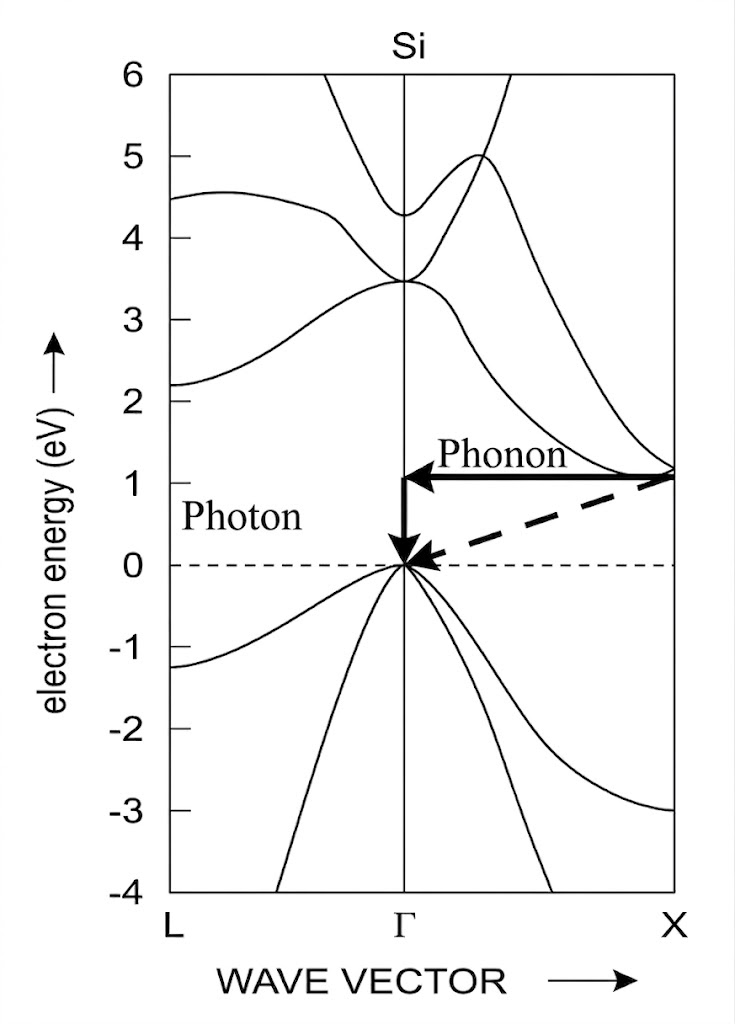
\includegraphics[width=\linewidth]{../Figures/Sheet 5/q5.jpg}
\end{minipage}
\end{question}

\textbf{\large Solution --- Question 5}

\textbf{Energy and momentum balances.}

In an indirect bandgap semiconductor like silicon, radiative transitions require the participation of a phonon to conserve momentum. The minimum of the conduction band sits at $k_x = 2\pi/a$, while the valence band maximum is at $k = 0$. The necessary momentum exchange with the lattice must be provided by the phonon:

\begin{equation*}
  p_{phonon} = \hbar \Delta k = \frac{h}{2\pi} \left( \frac{2\pi}{a} \right) = \frac{h}{a}
\end{equation*}

Given the lattice constant $a = 5.43$\,\AA:

\begin{equation*}
  \boxed{p_{phonon} = \frac{6.626\times10^{-34}}{5.43\times10^{-10}} \approx 1.22\times10^{-24}\,\text{kg}\cdot\text{m/s}.}
\end{equation*}

This momentum is identical regardless of whether the phonon is absorbed or emitted.

\textbf{(a) Photon emission by absorbing a phonon.}

By conservation of energy, the energy from the initial conduction state and the absorbed phonon is entirely transferred into the emitted photon and the final valence state:

\begin{equation*}
  E_2 + E_{phonon} = E_1 + E_{photon} \quad\Longrightarrow\quad E_{photon} = (E_2 - E_1) + E_{phonon}
\end{equation*}

Assuming transitions occur directly across the bandgap ($E_2 - E_1 \approx E_g$):

\begin{equation*}
  E_{photon} = 1.1\,\text{eV} + 0.03\,\text{eV} = 1.13\,\text{eV}
\end{equation*}

The resulting photon wavelength is:

\begin{equation*}
  \boxed{\lambda_a = \frac{hc}{E_{photon}} = \frac{1.24}{1.13} \approx 1.097\,\mu\text{m}.}
\end{equation*}

\textbf{(b) Photon emission by emitting a phonon.}

In this scenario, the transition energy is shared between both an emitted photon and an emitted phonon:

\begin{equation*}
  E_2 = E_1 + E_{photon} + E_{phonon} \quad\Longrightarrow\quad E_{photon} = (E_2 - E_1) - E_{phonon}
\end{equation*}

\begin{equation*}
  E_{photon} = 1.1\,\text{eV} - 0.03\,\text{eV} = 1.07\,\text{eV}
\end{equation*}

The resulting photon wavelength is:

\begin{equation*}
  \boxed{\lambda_b = \frac{hc}{E_{photon}} = \frac{1.24}{1.07} \approx 1.158\,\mu\text{m}.}
\end{equation*}

The difference between the two emitted wavelengths represents the substantial spectral shift caused by phonon interaction:

\begin{equation*}
  \boxed{\Delta\lambda_{ph} = \lambda_b - \lambda_a = 1.158 - 1.097 = 61\,\text{nm}.}
\end{equation*}

\begin{question}[Question 6]
(a) For a semiconductor in thermal equilibrium ($E_{fc} = E_{fv} = E_f$), show that $f_e(v)$ is always smaller than $f_a(v)$ so that the rate of photon emission cannot exceed the rate of photon absorption.\\
(b) For a semiconductor in quasi-equilibrium ($E_{fc} \neq E_{fv}$), with radiative transitions occurring between a conduction-band state of energy $E_2$, and a valence-band state of energy $E_1$ with the same $k$, show that emission is more likely than absorption if the separation between the quasi-Fermi levels is larger than the photon energy, i.e., if $E_{fc} - E_{fv} > h\nu$. What does this condition imply about the locations of $E_{fc}$ relative to $E_c$, and $E_{fv}$ relative to $E_v$?
\end{question}

\textbf{\large Solution --- Question 6}

\textbf{(a) Thermal equilibrium limits.}

The net gain probability function is the difference between the probability of emission and the probability of absorption. Under thermal equilibrium conditions ($E_{fc} = E_{fv} = E_f$):

\begin{equation*}
  f_g(\nu) = f_e(\nu) - f_a(\nu) = f(E_2) - f(E_1)
\end{equation*}

Substituting the Fermi-Dirac distributions:

\begin{equation*}
  f_g(\nu) = \frac{1}{1 + \exp\left(\frac{E_2 - E_f}{k_B T}\right)} - \frac{1}{1 + \exp\left(\frac{E_1 - E_f}{k_B T}\right)}
\end{equation*}

Because the conduction band state is always energetically higher than the valence band state ($E_2 > E_1$), it follows that the exponential denominator for $f(E_2)$ is strictly larger than for $f(E_1)$. Therefore:

\begin{equation*}
  f(E_2) < f(E_1) \quad\Longrightarrow\quad f_g(\nu) < 0
\end{equation*}

This firmly demonstrates that at thermal equilibrium, the rate of stimulated photon emission can never exceed the rate of photon absorption, preventing the material from acting as an optical amplifier.

\textbf{(b) Quasi-equilibrium and population inversion.}

Under quasi-equilibrium conditions caused by external pumping ($E_{fc} \neq E_{fv}$), achieving net amplification requires that $f_g(\nu) > 0$, or $f_c(E_2) > f_v(E_1)$:

\begin{equation*}
  \frac{1}{1 + \exp\left(\frac{E_2 - E_{fc}}{k_B T}\right)} > \frac{1}{1 + \exp\left(\frac{E_1 - E_{fv}}{k_B T}\right)}
\end{equation*}

For the inequality to hold, the exponent in the emission term must be strictly less than the absorption term:

\begin{equation*}
  \exp\left(\frac{E_1 - E_{fv}}{k_B T}\right) > \exp\left(\frac{E_2 - E_{fc}}{k_B T}\right) \quad\Longrightarrow\quad E_1 - E_{fv} > E_2 - E_{fc}
\end{equation*}

Rearranging these terms to group the quasi-Fermi levels and the transition energies:

\begin{equation*}
  E_{fc} - E_{fv} > E_2 - E_1
\end{equation*}

Since the transition energy is exactly the photon energy ($E_2 - E_1 = h\nu$), we obtain the Bernard-Duraffourg condition for optical gain:

\begin{equation*}
  \boxed{E_{fc} - E_{fv} > h\nu}
\end{equation*}

Physically, this condition demands that the quasi-Fermi separation exceed the bandgap itself ($h\nu \ge E_g$). This strongly implies that $E_{fc}$ must be driven high up into the conduction band ($E_{fc} > E_c$) and $E_{fv}$ pushed deep down into the valence band ($E_{fv} < E_v$), achieving full population inversion.

\begin{question}[Question 7]
Determine the free-space wavelength $\lambda_p$, at which the band-to-band absorption coefficient of a semiconductor in thermal equilibrium is maximum. Calculate the value of $\lambda_p$, for GaAs. Assume that $\tau_r = 0.4$ ns, $n = 3.6$, $m_e^* = 0.07 m_o$, $m_h^* = 0.5 m_o$, and $E_g = 1.42$ eV. Note that this result applies only to absorption by direct band-to-band transitions.
\end{question}

\textbf{\large Solution --- Question 7}

The absorption coefficient $\alpha(\nu)$ for direct band-to-band transitions is proportional to the joint density of states $\rho_j(\nu)$ and inversely proportional to the square of the optical frequency:

\begin{equation*}
  \alpha(\nu) = \frac{c^2}{8\pi n^2 \nu^2 \tau_{sp}} \rho_j(\nu)
\end{equation*}

Because the joint density of states $\rho_j(\nu)$ scales with $\sqrt{h\nu - E_g}$, the overall frequency dependence of the absorption coefficient takes the form:

\begin{equation*}
  \alpha(\nu) = \text{Const.} \times \frac{\sqrt{h\nu - E_g}}{\nu^2}
\end{equation*}

To find the frequency at which this absorption is maximized, we differentiate $\alpha$ with respect to $\nu$ and equate it to zero:

\begin{equation*}
  \frac{\partial \alpha}{\partial \nu} = \text{Const.} \left[ \frac{-2}{\nu^3} \sqrt{h\nu - E_g} + \frac{1}{\nu^2} \frac{h}{2\sqrt{h\nu - E_g}} \right] = 0
\end{equation*}

Multiplying through by $\nu^3 \sqrt{h\nu - E_g}$ to eliminate the denominators yields:

\begin{equation*}
  -2(h\nu - E_g) + \frac{h\nu}{2} = 0 \quad\Longrightarrow\quad 4(h\nu - E_g) = h\nu
\end{equation*}

\begin{equation*}
  3h\nu = 4E_g \quad\Longrightarrow\quad h\nu_p = \frac{4}{3} E_g
\end{equation*}

This defines the photon energy at which absorption peaks. To find the corresponding free-space wavelength $\lambda_p$, we use the fundamental relation $E = hc/\lambda_p$:

\begin{equation*}
  \frac{hc}{\lambda_p} = \frac{4}{3} E_g \quad\Longrightarrow\quad \lambda_p = \frac{3hc}{4E_g}
\end{equation*}

It is important to note that while the light propagates within a semiconductor of refractive index $n$, the \emph{free-space} wavelength $\lambda_p$ associated with the photon energy $E = h\nu$ does not depend on $n$. Only the local physical wavelength inside the crystal ($\lambda_{\text{medium}} = \lambda_p / n$) scales with the refractive index. Therefore, evaluating this strictly for free space:

For GaAs with a bandgap of $E_g = 1.42$\,eV, substituting the fundamental constants ($h = 6.626 \times 10^{-34}$\,J$\cdot$s, $c = 3 \times 10^8$\,m/s, and $1\,\text{eV} = 1.602 \times 10^{-19}$\,J):

\begin{equation*}
  \lambda_p = \frac{3 \times (6.626 \times 10^{-34}) \times (3 \times 10^8)}{4 \times (1.42 \times 1.602 \times 10^{-19})} \approx 6.55 \times 10^{-7}\,\text{m}
\end{equation*}

\begin{equation*}
  \boxed{\lambda_p = 655\,\text{nm}.}
\end{equation*}

\begin{question}[Question 8]
An important effect of heavy doping is the narrowing of the bandgap. This can have serious effects on the performance of different electronic and optoelectronic devices. In silicon, if $N_d$ is the donor density (in cm$^{-3}$), then the bandgap narrowing is given by the simple expression
\begin{equation*}
\Delta E_g \approx -22.5\sqrt{(N_d/10^{18})(300/T)} \text{ meV}
\end{equation*}
where $T$ is the temperature in Kelvin. This expression gives reasonable agreement with experiments at low doping levels. At high doping levels it over-estimates the bandgap narrowing. However, due to its simplicity we may use it to get an estimate of the bandgap narrowing. Use this expression to find the maximum wavelength of the photons that may be absorbed by an N-type silicon at room temperature at a donor concentration of $10^{18}$ cm$^{-3}$, $10^{19}$ cm$^{-3}$, and $10^{20}$ cm$^{-3}$.
\end{question}

\textbf{\large Solution --- Question 8}

At room temperature ($T = 300$\,K), the temperature-dependent factor simplifies to unity. The effective bandgap $E_g$ of the heavily doped silicon is the original undoped bandgap ($E_{g_o} \approx 1.10$\,eV for Si at 300\,K) minus the narrowing magnitude:

\begin{equation*}
  E_g = E_{g_o} + \Delta E_g
\end{equation*}

Because photons are only absorbed if their energy meets or exceeds the bandgap ($h\nu \ge E_g$), the maximum absorbed wavelength $\lambda_{\text{max}}$ directly corresponds to the narrowed bandgap energy:

\begin{equation*}
  E_g = \frac{1.24}{\lambda_{\text{max}}} \quad\Longrightarrow\quad \lambda_{\text{max}} = \frac{1.24}{E_g}
\end{equation*}

We evaluate this for the three given donor concentrations:

\textbf{Case 1: $N_d = 10^{18}\,\text{cm}^{-3}$}
\begin{equation*}
  \Delta E_g = -22.5 \sqrt{\frac{10^{18}}{10^{18}}} = -22.5\,\text{meV} = -0.0225\,\text{eV}
\end{equation*}
\begin{equation*}
  E_g = 1.10 - 0.0225 = 1.0775\,\text{eV} \quad\Longrightarrow\quad \boxed{\lambda_{\text{max}} = \frac{1.24}{1.0775} = 1.1508\,\mu\text{m}}
\end{equation*}

\textbf{Case 2: $N_d = 10^{19}\,\text{cm}^{-3}$}
\begin{equation*}
  \Delta E_g = -22.5 \sqrt{\frac{10^{19}}{10^{18}}} = -22.5\sqrt{10} \approx -71.15\,\text{meV} = -0.0712\,\text{eV}
\end{equation*}
\begin{equation*}
  E_g = 1.10 - 0.0712 = 1.0288\,\text{eV} \quad\Longrightarrow\quad \boxed{\lambda_{\text{max}} = \frac{1.24}{1.0288} = 1.205\,\mu\text{m}}
\end{equation*}

\textbf{Case 3: $N_d = 10^{20}\,\text{cm}^{-3}$}
\begin{equation*}
  \Delta E_g = -22.5 \sqrt{\frac{10^{20}}{10^{18}}} = -22.5\sqrt{100} = -225\,\text{meV} = -0.225\,\text{eV}
\end{equation*}
\begin{equation*}
  E_g = 1.10 - 0.225 = 0.875\,\text{eV} \quad\Longrightarrow\quad \boxed{\lambda_{\text{max}} = \frac{1.24}{0.875} = 1.417\,\mu\text{m}}
\end{equation*}

This demonstrates that heavier doping causes the absorption edge to shift significantly deeper into the infrared spectrum.

\begin{question}[Question 9]
(a) Use the gain coefficient ($\gamma = (\lambda^2/8\pi\tau_{sp}) f_g(\nu) \rho_j(\nu)$) of the semiconductor optical amplifier (SOA) to derive an expression of the amplifier bandwidth (where $\gamma$ is positive).\\
(b) Consider an InGaAsP SOA with an energy gap, $E_g = 0.95$ eV, a refractive index, $n = 3.5$, and a spontaneous emission lifetime, $\tau_{sp} = 2.5$ ns, at room temperature ($T = 300$ K). Calculate the amplifier bandwidth (in nanometers) under steady-state excess-carrier concentration, $\Delta n = 1.8 \times 10^{18}$ cm$^{-3}$.
\end{question}

\textbf{\large Solution --- Question 9}

\textbf{(a) Amplifier bandwidth expression.}

The gain coefficient $\gamma(\nu)$ is positive only when the Fermi inversion factor $f_g(\nu)$ is positive. This requires the photon energy $h\nu$ to be smaller than the quasi-Fermi level separation (the Bernard-Duraffourg condition). Furthermore, band-to-band transitions only exist for photon energies above the bandgap. Therefore, the frequency range that experiences optical gain is bounded by:

\begin{equation*}
  E_g < h\nu < E_{fc} - E_{fv}
\end{equation*}

The optical bandwidth (in Hz) is defined by the width of this energy window divided by Planck's constant:

\begin{equation*}
  BW = \frac{E_{fc} - E_{fv} - E_g}{h}
\end{equation*}

To express this in terms of carrier injection, we utilize the low-temperature (degenerate) approximation where the quasi-Fermi levels are related to the carrier concentration $\Delta n$. The total Fermi separation is:

\begin{equation*}
  E_{fc} - E_{fv} = E_g + (3\pi^2)^{2/3} \frac{\hbar^2}{2 m_e^*} (\Delta n)^{2/3} + (3\pi^2)^{2/3} \frac{\hbar^2}{2 m_h^*} (\Delta n)^{2/3}
\end{equation*}

Factoring out the common terms and using the reduced effective mass $m_r = (1/m_e^* + 1/m_h^*)^{-1}$:

\begin{equation*}
  E_{fc} - E_{fv} = E_g + (3\pi^2)^{2/3} \frac{\hbar^2}{2 m_r} (\Delta n)^{2/3}
\end{equation*}

Subtracting $E_g$ and dividing by $h$:

\begin{equation*}
  BW = \frac{1}{h} (3\pi^2)^{2/3} \frac{(h/2\pi)^2}{2 m_r} (\Delta n)^{2/3}
\end{equation*}

\begin{equation*}
  \boxed{BW = (3\pi^2)^{2/3} \frac{h}{8\pi^2 m_r} (\Delta n)^{2/3}}
\end{equation*}

\textbf{(b) Numerical calculation for InGaAsP SOA.}

First, we calculate the absolute energy bandwidth (the Fermi level separation). Assuming a representative reduced effective mass for these III-V materials ($m_r \approx 0.0614 m_o = 5.587 \times 10^{-32}$\,kg), we evaluate the quasi-Fermi level separation:

\begin{equation*}
  E_{fc} - E_{fv} = E_g + (3\pi^2)^{2/3} \frac{\hbar^2}{2 m_r} (\Delta n)^{2/3}
\end{equation*}

Converting the concentration to SI units: $\Delta n = 1.8 \times 10^{18}\,\text{cm}^{-3} = 1.8 \times 10^{24}\,\text{m}^{-3}$.

\begin{equation*}
  E_{fc} - E_{fv} = 0.95\,\text{eV} + \frac{9.587 \times (1.054 \times 10^{-34})^2}{2 \times 5.587 \times 10^{-32}} (1.8 \times 10^{24})^{2/3}\,\text{J}
\end{equation*}

\begin{equation*}
  E_{fc} - E_{fv} = 0.95\,\text{eV} + \frac{1.408 \times 10^{-20}\,\text{J}}{1.6 \times 10^{-19}\,\text{J/eV}} = 0.95\,\text{eV} + 0.088\,\text{eV} = 1.038\,\text{eV}
\end{equation*}

The equivalent frequency bandwidth is:

\begin{equation*}
  \boxed{BW = \frac{0.088\,\text{eV} \times 1.6 \times 10^{-19}\,\text{J/eV}}{6.626 \times 10^{-34}\,\text{J}\cdot\text{s}} \approx 21.27\,\text{THz}.}
\end{equation*}

The problem specifically asks for the bandwidth \emph{in nanometers}. We find the wavelengths corresponding to the edges of the gain spectrum:

\begin{equation*}
  \lambda_{\text{max}} = \frac{1.24}{E_g} = \frac{1.24}{0.95} = 1.305\,\mu\text{m} = 1305\,\text{nm}
\end{equation*}

\begin{equation*}
  \lambda_{\text{min}} = \frac{1.24}{E_{fc} - E_{fv}} = \frac{1.24}{1.038} \approx 1.1946\,\mu\text{m} \approx 1194.6\,\text{nm}
\end{equation*}

The wavelength bandwidth $\Delta \lambda$ is the difference:

\begin{equation*}
  \Delta \lambda = \lambda_{\text{max}} - \lambda_{\text{min}} = 1305 - 1194.6 = 110.4\,\text{nm}
\end{equation*}

\begin{equation*}
  \boxed{\Delta \lambda = 110.4\,\text{nm}.}
\end{equation*}

\begin{question}[Question 10]
Assume that electron-hole pairs are injected into n-type GaAs ($E_g = 1.42$ eV, $m_e^* = 0.07 m_o$, $m_h^* = 0.5 m_o$) at a rate $R = 10^{23}$ per cm$^3$ per second. The thermal equilibrium concentration of electrons is $n_o = 10^{16}$ cm$^{-3}$. If the recombination parameter $r = 10^{-11}$ cm$^3$/s and T = 300 K, determine:\\
(a) The equilibrium concentration of holes, $p_o$.\\
(b) The recombination lifetime $\tau$.\\
(c) The steady-state excess concentration $\Delta n$\\
(d) The separation between the quasi-Fermi levels $E_{fc} - E_{fv}$, assuming that $T = 0$ K.
\end{question}

\textbf{\large Solution --- Question 10}

\textbf{(a) Equilibrium hole concentration.}

We first evaluate the effective density of states for both the conduction and valence bands. Utilizing the standard expressions and converting the effective masses to kilograms ($m_o = 9.1 \times 10^{-31}$\,kg):

\begin{equation*}
  N_c = 2 \left( \frac{2\pi m_e^* k_B T}{h^2} \right)^{3/2} = 4.64 \times 10^{23}\,\text{m}^{-3} = 4.64 \times 10^{17}\,\text{cm}^{-3}
\end{equation*}

\begin{equation*}
  N_v = 2 \left( \frac{2\pi m_h^* k_B T}{h^2} \right)^{3/2} = 8.85 \times 10^{24}\,\text{m}^{-3} = 8.85 \times 10^{18}\,\text{cm}^{-3}
\end{equation*}

The intrinsic carrier concentration squared is given by the mass-action law:

\begin{equation*}
  n_i^2 = N_c N_v \exp\left(-\frac{E_g}{k_B T}\right) = (4.64\times 10^{17}) (8.85\times 10^{18}) \exp\left(-\frac{1.42}{0.0259}\right) = 6.022 \times 10^{12}\,\text{cm}^{-6}
\end{equation*}

Since the material is in thermal equilibrium, we can find the minority hole concentration $p_o$:

\begin{equation*}
  \boxed{p_o = \frac{n_i^2}{n_o} = \frac{6.022 \times 10^{12}}{10^{16}} = 6.022 \times 10^{-4}\,\text{cm}^{-3}.}
\end{equation*}

\textbf{(c) Steady-state excess concentration.}
\textit{(We solve part (c) first as it is required to find the lifetime in part (b)).}

The net recombination rate $R$ dictates the steady-state excess carrier concentration $\Delta n$. By definition:

\begin{equation*}
  R = r \Delta n (n_o + \Delta n) \quad\Longrightarrow\quad 10^{23} = 10^{-11} \left[ \Delta n^2 + 10^{16} \Delta n \right]
\end{equation*}

This forms a quadratic equation in terms of $\Delta n$:

\begin{equation*}
  \Delta n^2 + 10^{16} \Delta n - 10^{34} = 0
\end{equation*}

Solving via the quadratic formula and taking the positive physical root:

\begin{equation*}
  \boxed{\Delta n = \frac{-10^{16} + \sqrt{10^{32} + 4\times 10^{34}}}{2} = 9.512 \times 10^{16}\,\text{cm}^{-3}.}
\end{equation*}

\textbf{(b) Recombination lifetime.}

The minority carrier lifetime $\tau$ (often denoted $\tau_p$ for holes in an n-type material) is defined by the ratio of the excess concentration to the recombination rate:

\begin{equation*}
  \tau = \frac{\Delta n}{R} = \frac{9.512 \times 10^{16}}{10^{23}} = 9.512 \times 10^{-7}\,\text{s}
\end{equation*}

\begin{equation*}
  \boxed{\tau = 951.2\,\text{ns}.}
\end{equation*}

\textbf{(d) Quasi-Fermi level separation at absolute zero.}

At $T = 0$\,K, the semiconductor becomes heavily degenerate under injection, and the carrier concentrations are entirely given by the states filled up to the quasi-Fermi levels. The total separation is:

\begin{equation*}
  E_{fc} - E_{fv} = E_g + (E_{fc} - E_c) + (E_v - E_{fv})
\end{equation*}

Using the zero-temperature expressions derived previously, and recognizing that $\Delta n = n = p$ at absolute zero:

\begin{equation*}
  E_{fc} - E_{fv} = E_g + (3\pi^2)^{2/3} \frac{\hbar^2}{2 m_e^*} (\Delta n)^{2/3} + (3\pi^2)^{2/3} \frac{\hbar^2}{2 m_h^*} (\Delta n)^{2/3}
\end{equation*}

Factoring out the common terms and defining the reduced effective mass $m_r = \left(\frac{1}{m_e^*} + \frac{1}{m_h^*}\right)^{-1}$:

\begin{equation*}
  E_{fc} - E_{fv} = E_g + (3\pi^2)^{2/3} \frac{\hbar^2}{2 m_r} (\Delta n)^{2/3}
\end{equation*}

Given $m_r = \frac{0.07 \times 0.5}{0.07 + 0.5} m_o = 0.0614 m_o$ and $\Delta n = 9.512 \times 10^{16}$\,cm$^{-3} = 9.512 \times 10^{22}$\,m$^{-3}$:

\begin{equation*}
  \boxed{E_{fc} - E_{fv} = 1.4324\,\text{eV}.}
\end{equation*}


\begin{question}[Question 11]
(a) Determine the photon energy $\nu$, at which the direct band-to-band spontaneous emission rate from a semiconductor material in thermal equilibrium achieves its maximum value when the Fermi level lies within the bandgap and away from the band edges by at least several times $K_B T$.\\
(b) Show that this peak rate (photons per second per hertz per cm$^3$) is given by
\begin{equation*}
r_{sp}(\nu_p) = \frac{2(m_r)^{3/2}}{\pi\hbar^2\tau_r} \sqrt{\frac{K_B T}{e}} \exp\left(-\frac{E_g}{K_B T}\right)
\end{equation*}
(c) What is the effect of doping on this result?\\
(d) Assuming that $\tau_r = 0.4$ ns, $m_e^* = 0.07 m_o$, $m_h^* = 0.5 m_o$, and $E_g = 1.42$ eV, find the peak rate in GaAs at T = 300 K.
\end{question}

\textbf{\large Solution --- Question 11}

\textbf{(a) Peak spontaneous emission energy.}

The spontaneous emission rate as a function of frequency is the product of the emission probability $f_e(\nu)$ and the joint density of states $\rho_j(\nu)$, scaled by the spontaneous lifetime:

\begin{equation*}
  r_{sp}(\nu) = \frac{1}{\tau_{sp}} f_e(\nu) \rho_j(\nu)
\end{equation*}

For a non-degenerate semiconductor in thermal equilibrium, the emission probability function can be approximated using Boltzmann statistics:

\begin{equation*}
  f_e(\nu) = f(E_2)[1 - f(E_1)] \simeq \exp\left(-\frac{E_2 - E_f}{k_B T}\right) \exp\left(\frac{E_1 - E_f}{k_B T}\right) = \exp\left(-\frac{h\nu}{k_B T}\right)
\end{equation*}

We can also extract the bandgap energy from the exponent for mathematical convenience later:

\begin{equation*}
  f_e(\nu) = \exp\left(-\frac{h\nu - E_g}{k_B T}\right) \exp\left(-\frac{E_g}{k_B T}\right)
\end{equation*}

The joint density of states in terms of frequency is proportional to $\sqrt{h\nu - E_g}$. Thus, the overall rate proportionality is:

\begin{equation*}
  r_{sp}(\nu) = \text{Const} \times \sqrt{h\nu - E_g} \exp\left(-\frac{h\nu - E_g}{k_B T}\right)
\end{equation*}

To find the peak frequency $\nu_p$, we differentiate this rate with respect to $\nu$ and set it to zero:

\begin{equation*}
  \frac{\partial r_{sp}}{\partial \nu} = \text{Const} \times \left[ \frac{-h}{k_B T} \exp\left(-\frac{h\nu - E_g}{k_B T}\right) \sqrt{h\nu - E_g} + \frac{h}{2\sqrt{h\nu - E_g}} \exp\left(-\frac{h\nu - E_g}{k_B T}\right) \right] = 0
\end{equation*}

\begin{equation*}
  \frac{\sqrt{h\nu - E_g}}{k_B T} = \frac{1}{2\sqrt{h\nu - E_g}} \quad\Longrightarrow\quad h\nu - E_g = \frac{k_B T}{2}
\end{equation*}

\begin{equation*}
  \boxed{h\nu_p = E_g + \frac{k_B T}{2}}
\end{equation*}

\textbf{(b) Expression for the peak rate.}

The joint density of states expressed in terms of frequency is:

\begin{equation*}
  \rho_j(\nu) = \frac{2\sqrt{2} m_r^{3/2}}{\pi \hbar^2} \sqrt{h\nu - E_g}
\end{equation*}

Substituting this and our derived peak energy $h\nu_p$ into the spontaneous emission rate equation:

\begin{equation*}
  r_{sp}(\nu_p) = \frac{1}{\tau_{sp}} \exp\left(-\frac{h\nu_p}{k_B T}\right) \frac{2\sqrt{2} m_r^{3/2}}{\pi \hbar^2} \sqrt{h\nu_p - E_g}
\end{equation*}

Using $h\nu_p = E_g + k_B T/2$, the exponential term becomes $e^{-E_g / k_B T} e^{-1/2}$, and the square root term becomes $\sqrt{k_B T/2}$. Note that $e^{-1/2} = 1/\sqrt{e}$ where $e$ is Euler's number:

\begin{equation*}
  r_{sp}(\nu_p) = \frac{1}{\tau_{sp}} e^{-\frac{E_g}{k_B T}} e^{-1/2} \frac{2\sqrt{2} m_r^{3/2}}{\pi \hbar^2} \sqrt{\frac{k_B T}{2}} = \frac{1}{\tau_{sp}} e^{-\frac{E_g}{k_B T}} \frac{2 m_r^{3/2}}{\pi \hbar^2} \sqrt{\frac{k_B T}{e}}
\end{equation*}

Assuming the spontaneous lifetime $\tau_{sp}$ is equivalent to the radiative lifetime $\tau_r$:

\begin{equation*}
  \boxed{r_{sp}(\nu_p) = \frac{2 m_r^{3/2}}{\pi \hbar^2 \tau_r} \sqrt{\frac{k_B T}{e}} \exp\left(-\frac{E_g}{k_B T}\right)}
\end{equation*}

\textbf{(c) Effect of doping.}

Doping a semiconductor introduces a massive excess of majority carriers. Consequently, any injected minority carriers will encounter a much larger population of available opposite-charge carriers to recombine with. This significantly increases the overall recombination rate and correspondingly decreases the radiative lifetime ($\tau_r$). As our derived peak rate is inversely proportional to $\tau_r$, \textbf{doping causes the peak spontaneous emission rate to increase}.

\textbf{(d) Peak rate calculation for GaAs.}

First, we determine the reduced effective mass $m_r$:

\begin{equation*}
  m_r = \frac{m_e^* m_h^*}{m_e^* + m_h^*} = \frac{0.07 \times 0.5}{0.57} m_o = 0.0614 m_o \approx 5.587 \times 10^{-32}\,\text{kg}
\end{equation*}

Plugging in the physical constants at $T = 300$\,K:

\begin{equation*}
  r_{sp}(\nu_p) = \frac{2(5.587\times 10^{-32})^{3/2}}{\pi(1.054\times 10^{-34})^2 (0.4\times 10^{-9})} \sqrt{\frac{1.38\times 10^{-23} \times 300}{2.718}} \exp\left(-\frac{1.42}{0.0259}\right)
\end{equation*}

\begin{equation*}
  \boxed{r_{sp}(\nu_p) = 1.4 \times 10^{-4}\,\text{photons/s}\cdot\text{Hz}\cdot\text{cm}^3.}
\end{equation*}

\begin{question}[Question 12]
(a) Show that the direct band-to-band spontaneous emission rate integrated over all emission frequencies (photons per second per cm$^3$) is given by
\begin{equation*}
\int r_{sp}(\nu) d\nu = \frac{(m_r)^{3/2}}{\sqrt{2}\pi^{3/2}\hbar^3\tau_r} (K_B T)^{3/2} \exp\left(-\frac{E_g}{K_B T}\right)
\end{equation*}
provided that the Fermi level is within the semiconductor energy gap and away from the band edges. [Note: $\int_0^\infty \sqrt{x} e^{-\mu x} dx = \sqrt{\pi/4\mu^3}$]\\
(b) Compare this with the approximate integrated rate obtained by multiplying the peak rate obtained in Problem (5) by the approximate frequency width $2K_B T/h$ (the approximate width of $r_{sp}(\nu)$ as a function of frequency, $\nu$).\\
(c) Using the mass action law ($np = n_i^2$), set the phenomenological equilibrium radiative recombination rate, $rnp = rn_i^2$ (photons per second per cm$^3$) equal to the direct band-to-band result derived in (a) to obtain the expression for the radiative recombination rate
\begin{equation*}
r = \frac{\sqrt{2}\pi^{3/2}\hbar^3}{(m_e^* + m_h^*)^{3/2}} \frac{1}{(K_B T)^{3/2}\tau_r}
\end{equation*}
(d) Use the result in (c) to find the value of $r$, for GaAs at T = 300 K using $m_e^* = 0.07 m_o$, $m_h^* = 0.5 m_o$, and $\tau_r = 0.4$ ns.
\end{question}

\textbf{\large Solution --- Question 12}

\textbf{(a) Integrated spontaneous emission rate.}

We integrate the spontaneous emission rate function derived previously over all possible emission frequencies:

\begin{equation*}
  \int_{0}^{\infty} r_{sp}(\nu)\,d\nu = \int_{E_g/h}^{\infty} \frac{1}{\tau_{sp}} \exp\left(-\frac{E_g}{k_B T}\right) \exp\left(-\frac{h\nu - E_g}{k_B T}\right) \frac{2\sqrt{2} m_r^{3/2}}{\pi \hbar^2} \sqrt{h\nu - E_g}\,d\nu
\end{equation*}

We perform a change of variables, letting $x = \frac{h\nu - E_g}{k_B T}$. The differential becomes $d\nu = \frac{k_B T}{h} dx$:

\begin{equation*}
  \int_{0}^{\infty} r_{sp}(\nu)\,d\nu = \frac{1}{\tau_{sp}} e^{-\frac{E_g}{k_B T}} \frac{2\sqrt{2} m_r^{3/2}}{\pi \hbar^2} \int_{0}^{\infty} \sqrt{k_B T x} e^{-x} \left(\frac{k_B T}{h}\right) dx
\end{equation*}

Isolating the constants outside the integral:

\begin{equation*}
  \int_{0}^{\infty} r_{sp}(\nu)\,d\nu = \frac{1}{\tau_{sp}} e^{-\frac{E_g}{k_B T}} \frac{2\sqrt{2} m_r^{3/2}}{\pi \hbar^2} \frac{(k_B T)^{3/2}}{h} \int_{0}^{\infty} \sqrt{x} e^{-x} dx
\end{equation*}

Using the provided standard integral result $\int_0^\infty \sqrt{x} e^{-x} dx = \frac{\sqrt{\pi}}{2}$ and recognizing that $h = 2\pi\hbar$:

\begin{equation*}
  \int_{0}^{\infty} r_{sp}(\nu)\,d\nu = \frac{1}{\tau_{sp}} e^{-\frac{E_g}{k_B T}} \frac{2\sqrt{2} m_r^{3/2}}{\pi \hbar^2} \frac{(k_B T)^{3/2}}{2\pi\hbar} \left(\frac{\sqrt{\pi}}{2}\right)
\end{equation*}

Simplifying the numerical coefficients:

\begin{equation*}
  \boxed{\int_{0}^{\infty} r_{sp}(\nu)\,d\nu = \frac{m_r^{3/2}}{\sqrt{2} \pi^{3/2} \hbar^3 \tau_r} (k_B T)^{3/2} \exp\left(-\frac{E_g}{k_B T}\right)}
\end{equation*}

\textbf{(b) Comparison with the approximation.}

The approximate integrated rate assumes a rectangular spectral profile defined by the peak rate and an effective spectral width of $2k_B T/h$:

\begin{equation*}
  r_{sp,\text{approx}} = r_{sp}(\nu_p) \times \frac{2 k_B T}{h} = \left[ \frac{2 m_r^{3/2}}{\pi \hbar^2 \tau_r} \sqrt{\frac{k_B T}{e}} \exp\left(-\frac{E_g}{k_B T}\right) \right] \frac{2 k_B T}{2\pi\hbar}
\end{equation*}

\begin{equation*}
  r_{sp,\text{approx}} = \frac{2 m_r^{3/2}}{\pi^2 \hbar^3 \tau_r \sqrt{e}} (k_B T)^{3/2} \exp\left(-\frac{E_g}{k_B T}\right)
\end{equation*}

To compare this against the actual exact integral, we take the ratio:

\begin{equation*}
  \frac{r_{sp,\text{approx}}}{r_{sp,\text{actual}}} = \frac{\frac{2}{\pi^2 \sqrt{e}}}{\frac{1}{\sqrt{2} \pi^{3/2}}} = \frac{2\sqrt{2}}{\sqrt{\pi e}} = \sqrt{\frac{8}{\pi e}} \approx 0.968
\end{equation*}

\begin{equation*}
  \boxed{\text{Ratio} \approx 0.968.}
\end{equation*}

This demonstrates that the rectangular approximation is exceptionally accurate, underestimating the true integrated rate by only about 3.2\%.

\textbf{(c) Equilibrium radiative recombination parameter.}

By definition, the macroscopic recombination rate at thermal equilibrium is balanced by the thermal generation rate, governed by the recombination parameter $r$ and the intrinsic carrier concentration squared ($n_i^2$). We equate this to our microscopically derived exact integral:

\begin{equation*}
  r n_i^2 = \frac{m_r^{3/2}}{\sqrt{2} \pi^{3/2} \hbar^3 \tau_r} (k_B T)^{3/2} \exp\left(-\frac{E_g}{k_B T}\right)
\end{equation*}

We expand $n_i^2$ using the effective density of states $N_c$ and $N_v$:

\begin{equation*}
  n_i^2 = N_c N_v \exp\left(-\frac{E_g}{k_B T}\right) = 4 \left( \frac{2\pi k_B T}{h^2} \right)^3 (m_e^* m_h^*)^{3/2} \exp\left(-\frac{E_g}{k_B T}\right)
\end{equation*}

We can rewrite the $(2\pi k_B T / h^2)^3$ term by expanding $h = 2\pi\hbar$:

\begin{equation*}
  4 \left( \frac{2\pi k_B T}{4\pi^2\hbar^2} \right)^3 = 4 \left( \frac{k_B T}{2\pi\hbar^2} \right)^3 = \frac{(k_B T)^3}{2 \pi^3 \hbar^6}
\end{equation*}

Substituting this back into the equality, the exponential gap terms cancel out:

\begin{equation*}
  r \left[ \frac{(k_B T)^3}{2 \pi^3 \hbar^6} (m_e^* m_h^*)^{3/2} \right] = \frac{1}{\sqrt{2} \pi^{3/2} \hbar^3 \tau_r} (k_B T)^{3/2} \left( \frac{m_e^* m_h^*}{m_e^* + m_h^*} \right)^{3/2}
\end{equation*}

The $(m_e^* m_h^*)^{3/2}$ terms cancel on both sides. Solving for $r$:

\begin{equation*}
  r = \frac{2 \pi^3 \hbar^6}{\sqrt{2} \pi^{3/2} \hbar^3 (k_B T)^{3/2} \tau_r (m_e^* + m_h^*)^{3/2}}
\end{equation*}

\begin{equation*}
  \boxed{r = \frac{\sqrt{2}\pi^{3/2}\hbar^3}{(m_e^* + m_h^*)^{3/2}} \frac{1}{(k_B T)^{3/2}\tau_r}}
\end{equation*}

\textbf{(d) Value of the parameter $r$ for GaAs.}

We substitute the given material constants at $T = 300$\,K into our derived expression. The sum of the effective masses is $m_e^* + m_h^* = (0.07 + 0.5)m_o = 0.57 \times 9.1 \times 10^{-31} = 5.187 \times 10^{-31}$\,kg:

\begin{equation*}
  r = \frac{\sqrt{2} \pi^{3/2} (1.054 \times 10^{-34})^3}{(5.187 \times 10^{-31})^{3/2} (1.38 \times 10^{-23} \times 300)^{3/2} (0.4 \times 10^{-9})}
\end{equation*}

Evaluating the numerical components:

\begin{equation*}
  r = \frac{1.414 \times 5.568 \times 1.171 \times 10^{-102}}{1.182 \times 10^{-46} \times 2.664 \times 10^{-31} \times 4 \times 10^{-10}} \approx \frac{9.22 \times 10^{-102}}{1.26 \times 10^{-86}} \approx 7.3 \times 10^{-16}\,\text{m}^3/\text{s}
\end{equation*}

Converting this volumetric rate parameter to standard semiconductor units ($\text{cm}^3$/s):

\begin{equation*}
  \boxed{r = 7.3 \times 10^{-10}\,\text{cm}^3/\text{s}.}
\end{equation*}

\begin{question}[Formative Assignment Problem]
Show that the average kinetic energy of electrons in non-degenerate semiconductors which obeys the classical Boltzman statistics at thermal equilibrium is $3K_B T/2$. Find their average and root-mean square electron velocities in this case. Use the uncertainty principle to get an expression for their corresponding De Broglie wavelength at room temperature. (Hint: $\int_0^\infty x^{3/2} e^{-x} dx = \frac{3}{2}\int_0^\infty x^{1/2} e^{-x} dx$)
\end{question}

\textbf{\large Solution --- Formative Assignment}

\textbf{1. Average Kinetic Energy}

In a non-degenerate semiconductor, the electron distribution in the conduction band is well-described by the Maxwell-Boltzmann approximation. The average kinetic energy $\langle E_{kin} \rangle = \langle E - E_c \rangle$ is found by integrating the energy over the distribution of electrons, weighted by the density of states $\rho_c(E)$ and the Fermi-Dirac probability $f(E)$:

\begin{equation*}
  \langle E_{kin} \rangle = \frac{\int_{E_c}^{\infty} (E - E_c) \rho_c(E) f(E)\,dE}{\int_{E_c}^{\infty} \rho_c(E) f(E)\,dE}
\end{equation*}

The conduction band density of states scales as $\rho_c(E) \propto \sqrt{E - E_c}$, and the Boltzmann probability is $f(E) \propto \exp\left(-\frac{E - E_c}{k_B T}\right)$. Substituting these proportionalities:

\begin{equation*}
  \langle E_{kin} \rangle = \frac{\int_{E_c}^{\infty} (E - E_c)^{3/2} \exp\left(-\frac{E - E_c}{k_B T}\right) dE}{\int_{E_c}^{\infty} (E - E_c)^{1/2} \exp\left(-\frac{E - E_c}{k_B T}\right) dE}
\end{equation*}

We introduce a dimensionless change of variables: let $x = \frac{E - E_c}{k_B T}$, meaning $E - E_c = x k_B T$ and $dE = k_B T dx$.

\begin{equation*}
  \langle E_{kin} \rangle = \frac{\int_{0}^{\infty} (x k_B T)^{3/2} e^{-x} (k_B T dx)}{\int_{0}^{\infty} (x k_B T)^{1/2} e^{-x} (k_B T dx)} = k_B T \frac{\int_{0}^{\infty} x^{3/2} e^{-x} dx}{\int_{0}^{\infty} x^{1/2} e^{-x} dx}
\end{equation*}

Using the provided integration identity $\int_0^\infty x^{3/2} e^{-x} dx = \frac{3}{2} \int_0^\infty x^{1/2} e^{-x} dx$, the integrals cancel exactly:

\begin{equation*}
  \boxed{\langle E_{kin} \rangle = \frac{3}{2} k_B T}
\end{equation*}

\textbf{2. Average and Root-Mean-Square Velocities}

The kinetic energy of an electron with an effective mass $m_e^*$ is $E_{kin} = \frac{1}{2} m_e^* v^2$. The root-mean-square (RMS) velocity characterizes the standard deviation of the velocity distribution and connects directly to the average kinetic energy:

\begin{equation*}
  \frac{1}{2} m_e^* v_{rms}^2 = \langle E_{kin} \rangle = \frac{3}{2} k_B T \quad\Longrightarrow\quad \boxed{v_{rms} = \sqrt{\frac{3 k_B T}{m_e^*}}}
\end{equation*}

To find the average absolute speed $\langle v \rangle$, we use the full 3D Maxwell-Boltzmann speed distribution $f(v)$:

\begin{equation*}
  \langle v \rangle = \int_0^\infty v f(v) dv = \int_0^\infty v \left[ 4\pi \left(\frac{m_e^*}{2\pi k_B T}\right)^{3/2} v^2 \exp\left(-\frac{m_e^* v^2}{2 k_B T}\right) \right] dv
\end{equation*}

\begin{equation*}
  \langle v \rangle = 4\pi \left(\frac{m_e^*}{2\pi k_B T}\right)^{3/2} \int_0^\infty v^3 \exp\left(-\frac{m_e^* v^2}{2 k_B T}\right) dv
\end{equation*}

The standard integral $\int_0^\infty v^3 e^{-a v^2} dv = \frac{1}{2a^2}$. Here, $a = \frac{m_e^*}{2 k_B T}$. Thus:

\begin{equation*}
  \langle v \rangle = 4\pi \left(\frac{m_e^*}{2\pi k_B T}\right)^{3/2} \frac{1}{2} \left(\frac{2 k_B T}{m_e^*}\right)^2 = \frac{4\pi}{2\pi\sqrt{2\pi}} \left(\frac{m_e^*}{k_B T}\right)^{3/2} \left(\frac{k_B T}{m_e^*}\right)^2 = \frac{2}{\sqrt{2\pi}} \sqrt{\frac{k_B T}{m_e^*}}
\end{equation*}

\begin{equation*}
  \boxed{\langle v \rangle = \sqrt{\frac{8 k_B T}{\pi m_e^*}}}
\end{equation*}

\textbf{3. Thermal de Broglie Wavelength}

The Heisenberg uncertainty principle states $\Delta x \Delta p \approx h$. At thermal equilibrium, the thermal momentum uncertainty of an electron limits how well its position can be resolved, effectively dictating its wave-packet size. Taking the momentum magnitude to be roughly $p \approx p_{rms} = m_e^* v_{rms} = \sqrt{3 m_e^* k_B T}$, the uncertainty principle yields the thermal de Broglie wavelength:

\begin{equation*}
  \lambda_{dB} \approx \Delta x \approx \frac{h}{\Delta p} = \frac{h}{p_{rms}}
\end{equation*}

\begin{equation*}
  \boxed{\lambda_{dB} = \frac{h}{\sqrt{3 m_e^* k_B T}}}
\end{equation*}
